\documentclass[12pt]{article}
%%%%%%%%%%%%%%%%
% Packages
%%%%%%%%%%%%%%%%

\usepackage[top=1cm,bottom=1.1cm,left=1.25cm,right= 1.25cm]{geometry}
\usepackage[parfill]{parskip}
\usepackage{graphicx, fontspec, xcolor,multicol, enumitem, setspace, amsmath, changepage}
\DeclareGraphicsRule{.tif}{png}{.png}{`convert #1 `dirname #1`/`basename #1 .tif`.png}

%%%%%%%%%%%%%%%%
% User defined colors
%%%%%%%%%%%%%%%%

% Pantone 2015 Fall colors
% http://iwork3.us/2015/02/18/pantone-2015-fall-fashion-report/
% update each semester or year

\xdefinecolor{custom_blue}{rgb}{0, 0.32, 0.48} % FROM SPRING 2016 COLOR PREVIEW
\xdefinecolor{custom_darkBlue}{rgb}{0.20, 0.20, 0.39} % Reflecting Pond  
\xdefinecolor{custom_orange}{rgb}{0.96, 0.57, 0.42} % Cadmium Orange
\xdefinecolor{custom_green}{rgb}{0, 0.47, 0.52} % Biscay Bay
\xdefinecolor{custom_red}{rgb}{0.58, 0.32, 0.32} % Marsala

\xdefinecolor{custom_lightGray}{rgb}{0.78, 0.80, 0.80} % Glacier Gray
\xdefinecolor{custom_darkGray}{rgb}{0.35, 0.39, 0.43} % Stormy Weather

%%%%%%%%%%%%%%%%
% Color text commands
%%%%%%%%%%%%%%%%

%orange
\newcommand{\orange}[1]{\textit{\textcolor{custom_orange}{#1}}}

% yellow
\newcommand{\yellow}[1]{\textit{\textcolor{yellow}{#1}}}

% blue
\newcommand{\blue}[1]{\textit{\textcolor{blue}{#1}}}

% green
\newcommand{\green}[1]{\textit{\textcolor{custom_green}{#1}}}

% red
\newcommand{\red}[1]{\textit{\textcolor{custom_red}{#1}}}

%%%%%%%%%%%%%%%%
% Coloring titles, links, etc.
%%%%%%%%%%%%%%%%

\usepackage{titlesec}
\titleformat{\section}
{\color{custom_blue}\normalfont\Large\bfseries}
{\color{custom_blue}\thesection}{1em}{}
\titleformat{\subsection}
{\color{custom_blue}\normalfont}
{\color{custom_blue}\thesubsection}{1em}{}

\newcommand{\ttl}[1]{ \textsc{{\LARGE \textbf{{\color{custom_blue} #1} } }}}

\newcommand{\tl}[1]{ \textsc{{\large \textbf{{\color{custom_blue} #1} } }}}

\usepackage[colorlinks=false,pdfborder={0 0 0},urlcolor= custom_orange,colorlinks=true,linkcolor= custom_orange, citecolor= custom_orange,backref=true]{hyperref}

%%%%%%%%%%%%%%%%
% Instructions box
%%%%%%%%%%%%%%%%

\newcommand{\inst}[1]{
\colorbox{custom_blue!20!white!50}{\parbox{\textwidth}{
	\vskip10pt
	\leftskip10pt \rightskip10pt
	#1
	\vskip10pt
}}
\vskip10pt
}
\usepackage{amsmath, amssymb}

%%%%%%%%%%%
% App Ex number    %
%%%%%%%%%%%

% DON'T FORGET TO UPDATE

%\newcommand{\appno}[1]
%{2.2}

%%%%%%%%%%%%%%
% Turn on/off solutions       %
%%%%%%%%%%%%%%

% Off
\newcommand{\soln}[2]{$\:$\\ \vspace{#1}}{}

%%%%%%%%%%%%%%%%
% Document
%%%%%%%%%%%%%%%%

\begin{document}
\fontspec[Ligatures=TeX]{Helvetica Neue Light}

Dr. Monod \hfill Sta 101: Data Analysis and Statistical Inference \\
Duke University -- Department of Statistical Science \hfill \\

\ttl{User Guide for i>clicker 2}

This document provides basic usage instructions for the i>clicker 2 (from now on referred to as ``clicker"), a required material for STA101.  The i>clicker 2 system is an interactive means to provide immediate and real-time feedback on course material during lectures; the clicker is a handheld device (remote) that allows students to respond anonymously (to other students) to questions asked in class, and allows the instructor to review the answers and provide real-time feedback and track the students' understanding of the material.  Clickers are used in this course to track participation in the course which count towards your grade, as well as for the multiple choice Readiness Assessments (RA) which take place at the beginning of each unit.

\section{Using the clicker in class to respond to multiple choice clicker questions (on lecture slides)}
\begin{enumerate}

\item Turn on the clicker by pressing the blue On/Off Power button on the remote and ensure that the screen reads READY.

\begin{center}
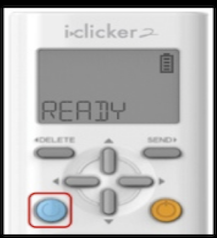
\includegraphics{clicker_images/clicker_ready.png}
\end{center}

\item When the polling session has begun, indicated by the following toolbar on the presentation slides,

\begin{center}
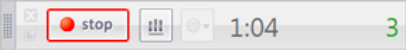
\includegraphics{clicker_images/polling.png}
\end{center}

select your answer from the available options, indicated on the slide, by pressing the corresponding A-E button on the remote.

\begin{center}
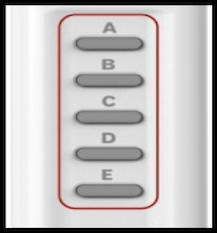
\includegraphics{clicker_images/buttons.png}
\end{center}

Your answer, indicated by a letter in the lower left corner of the clicker display, has been sent and registered when you see a check mark ($\checkmark$) in the upper right corner of the LCD clicker display, next to the battery icon.  Usually, simply clicking on one answer choice A-E on the clicker automatically sends the answer.

\begin{center}
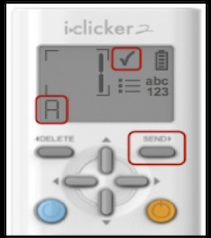
\includegraphics{clicker_images/send.png}
\end{center}

\item You can change your answer as many times as you like until the time is up. Only your last response will be recorded.

\item If you do not see the check mark ($\checkmark$), click the Send button to send your answer. The checkmark ($\checkmark$) indicates that your answer has been sent.

\end{enumerate}

\section{Using the clicker in class to respond to numerical clicker questions (on lecture slides)}

\section{Using the clicker during RAs}

\begin{enumerate}

\item Turn on the clicker by pressing the blue On/Off Power button on the remote and ensure that the screen reads READY.

\begin{center}
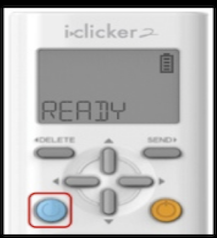
\includegraphics{clicker_images/clicker_ready.png}
\end{center}

\item When the self-paced polling session has begun, indicated by the following toolbar on the presentation slides,

\begin{center}
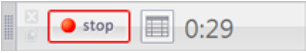
\includegraphics{clicker_images/self_polling.png}
\end{center}

select your answer from the available options, indicated on the RA handout, by pressing the corresponding A-E button on the remote.

\begin{center}
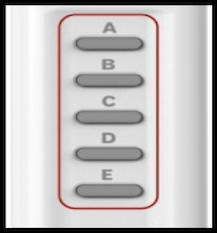
\includegraphics{clicker_images/buttons.png}
\end{center}

Your answer, indicated by a letter in the lower left corner of the clicker display, has been sent and registered when you see a check mark ($\checkmark$) in the upper right corner of the LCD clicker display, next to the battery icon.  Usually, simply clicking on one answer choice A-E on the clicker automatically sends the answer.

\begin{center}
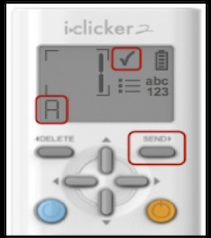
\includegraphics{clicker_images/send.png}
\end{center}

\item If you do not see the check mark ($\checkmark$), click the Send button. The checkmark ($\checkmark$) indicates that your answer has been sent.

\item Scroll between questions by clicking on the Up and Down arrows; Up moves to the next question, Down goes back to the previous question.  The question number is indicated in the large square on the upper left corner of the LCD clicker display.

\begin{center}
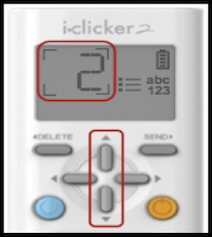
\includegraphics{clicker_images/switch.png}
\end{center}

\item You may scroll through the questions and change your answers as often you would like within the duration of the self-paced polling session, by following steps (2)-(4) above.  If a check mark ($\checkmark$) appears in the upper right corner of the LCD clicker display, then the corresponding answer found in the lower left corner of the LCD clicker display has been sent and registered.  You may change your answer simply by selecting another option A-E, and checking for the check mark ($\checkmark$).

\item Note that the self-paced polling session time counter counts up.  You have 15 minutes to complete an RA; the allowed time for the RA is complete when the time counter displays 15:00.

\end{enumerate}

\section{Trouble-shooting: Setting the frequency}

If, on your clicker display, you see the message SET FREQUENCY instead of READY:
\begin{enumerate}
\item Press and hold the blue On/Off Power button on the remote until the two-digit frequency on the LCD clicker display begins flashing.
\item Press A twice (AA) from the multiple choice buttons A-E on the remote.

\begin{center}
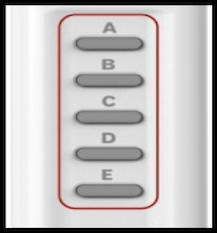
\includegraphics{clicker_images/buttons.png}
\end{center}

A check mark ($\checkmark$) appears on your remote indicating that you have successfully reset the remote frequency.  If you see this message, you will only have to set the frequency once and the frequency will remain set for the entirety of the course.
\end{enumerate}
\end{document}